% Options for packages loaded elsewhere
\PassOptionsToPackage{unicode}{hyperref}
\PassOptionsToPackage{hyphens}{url}
%
\documentclass[
]{article}
\usepackage{lmodern}
\usepackage{amsmath}
\usepackage{ifxetex,ifluatex}
\ifnum 0\ifxetex 1\fi\ifluatex 1\fi=0 % if pdftex
  \usepackage[T1]{fontenc}
  \usepackage[utf8]{inputenc}
  \usepackage{textcomp} % provide euro and other symbols
  \usepackage{amssymb}
\else % if luatex or xetex
  \usepackage{unicode-math}
  \defaultfontfeatures{Scale=MatchLowercase}
  \defaultfontfeatures[\rmfamily]{Ligatures=TeX,Scale=1}
\fi
% Use upquote if available, for straight quotes in verbatim environments
\IfFileExists{upquote.sty}{\usepackage{upquote}}{}
\IfFileExists{microtype.sty}{% use microtype if available
  \usepackage[]{microtype}
  \UseMicrotypeSet[protrusion]{basicmath} % disable protrusion for tt fonts
}{}
\makeatletter
\@ifundefined{KOMAClassName}{% if non-KOMA class
  \IfFileExists{parskip.sty}{%
    \usepackage{parskip}
  }{% else
    \setlength{\parindent}{0pt}
    \setlength{\parskip}{6pt plus 2pt minus 1pt}}
}{% if KOMA class
  \KOMAoptions{parskip=half}}
\makeatother
\usepackage{xcolor}
\IfFileExists{xurl.sty}{\usepackage{xurl}}{} % add URL line breaks if available
\IfFileExists{bookmark.sty}{\usepackage{bookmark}}{\usepackage{hyperref}}
\hypersetup{
  pdftitle={Shale gas},
  pdfauthor={Andrew J. Sims},
  hidelinks,
  pdfcreator={LaTeX via pandoc}}
\urlstyle{same} % disable monospaced font for URLs
\usepackage[margin=1in]{geometry}
\usepackage{color}
\usepackage{fancyvrb}
\newcommand{\VerbBar}{|}
\newcommand{\VERB}{\Verb[commandchars=\\\{\}]}
\DefineVerbatimEnvironment{Highlighting}{Verbatim}{commandchars=\\\{\}}
% Add ',fontsize=\small' for more characters per line
\usepackage{framed}
\definecolor{shadecolor}{RGB}{248,248,248}
\newenvironment{Shaded}{\begin{snugshade}}{\end{snugshade}}
\newcommand{\AlertTok}[1]{\textcolor[rgb]{0.94,0.16,0.16}{#1}}
\newcommand{\AnnotationTok}[1]{\textcolor[rgb]{0.56,0.35,0.01}{\textbf{\textit{#1}}}}
\newcommand{\AttributeTok}[1]{\textcolor[rgb]{0.77,0.63,0.00}{#1}}
\newcommand{\BaseNTok}[1]{\textcolor[rgb]{0.00,0.00,0.81}{#1}}
\newcommand{\BuiltInTok}[1]{#1}
\newcommand{\CharTok}[1]{\textcolor[rgb]{0.31,0.60,0.02}{#1}}
\newcommand{\CommentTok}[1]{\textcolor[rgb]{0.56,0.35,0.01}{\textit{#1}}}
\newcommand{\CommentVarTok}[1]{\textcolor[rgb]{0.56,0.35,0.01}{\textbf{\textit{#1}}}}
\newcommand{\ConstantTok}[1]{\textcolor[rgb]{0.00,0.00,0.00}{#1}}
\newcommand{\ControlFlowTok}[1]{\textcolor[rgb]{0.13,0.29,0.53}{\textbf{#1}}}
\newcommand{\DataTypeTok}[1]{\textcolor[rgb]{0.13,0.29,0.53}{#1}}
\newcommand{\DecValTok}[1]{\textcolor[rgb]{0.00,0.00,0.81}{#1}}
\newcommand{\DocumentationTok}[1]{\textcolor[rgb]{0.56,0.35,0.01}{\textbf{\textit{#1}}}}
\newcommand{\ErrorTok}[1]{\textcolor[rgb]{0.64,0.00,0.00}{\textbf{#1}}}
\newcommand{\ExtensionTok}[1]{#1}
\newcommand{\FloatTok}[1]{\textcolor[rgb]{0.00,0.00,0.81}{#1}}
\newcommand{\FunctionTok}[1]{\textcolor[rgb]{0.00,0.00,0.00}{#1}}
\newcommand{\ImportTok}[1]{#1}
\newcommand{\InformationTok}[1]{\textcolor[rgb]{0.56,0.35,0.01}{\textbf{\textit{#1}}}}
\newcommand{\KeywordTok}[1]{\textcolor[rgb]{0.13,0.29,0.53}{\textbf{#1}}}
\newcommand{\NormalTok}[1]{#1}
\newcommand{\OperatorTok}[1]{\textcolor[rgb]{0.81,0.36,0.00}{\textbf{#1}}}
\newcommand{\OtherTok}[1]{\textcolor[rgb]{0.56,0.35,0.01}{#1}}
\newcommand{\PreprocessorTok}[1]{\textcolor[rgb]{0.56,0.35,0.01}{\textit{#1}}}
\newcommand{\RegionMarkerTok}[1]{#1}
\newcommand{\SpecialCharTok}[1]{\textcolor[rgb]{0.00,0.00,0.00}{#1}}
\newcommand{\SpecialStringTok}[1]{\textcolor[rgb]{0.31,0.60,0.02}{#1}}
\newcommand{\StringTok}[1]{\textcolor[rgb]{0.31,0.60,0.02}{#1}}
\newcommand{\VariableTok}[1]{\textcolor[rgb]{0.00,0.00,0.00}{#1}}
\newcommand{\VerbatimStringTok}[1]{\textcolor[rgb]{0.31,0.60,0.02}{#1}}
\newcommand{\WarningTok}[1]{\textcolor[rgb]{0.56,0.35,0.01}{\textbf{\textit{#1}}}}
\usepackage{longtable,booktabs}
\usepackage{calc} % for calculating minipage widths
% Correct order of tables after \paragraph or \subparagraph
\usepackage{etoolbox}
\makeatletter
\patchcmd\longtable{\par}{\if@noskipsec\mbox{}\fi\par}{}{}
\makeatother
% Allow footnotes in longtable head/foot
\IfFileExists{footnotehyper.sty}{\usepackage{footnotehyper}}{\usepackage{footnote}}
\makesavenoteenv{longtable}
\usepackage{graphicx}
\makeatletter
\def\maxwidth{\ifdim\Gin@nat@width>\linewidth\linewidth\else\Gin@nat@width\fi}
\def\maxheight{\ifdim\Gin@nat@height>\textheight\textheight\else\Gin@nat@height\fi}
\makeatother
% Scale images if necessary, so that they will not overflow the page
% margins by default, and it is still possible to overwrite the defaults
% using explicit options in \includegraphics[width, height, ...]{}
\setkeys{Gin}{width=\maxwidth,height=\maxheight,keepaspectratio}
% Set default figure placement to htbp
\makeatletter
\def\fps@figure{htbp}
\makeatother
\setlength{\emergencystretch}{3em} % prevent overfull lines
\providecommand{\tightlist}{%
  \setlength{\itemsep}{0pt}\setlength{\parskip}{0pt}}
\setcounter{secnumdepth}{-\maxdimen} % remove section numbering
\ifluatex
  \usepackage{selnolig}  % disable illegal ligatures
\fi
\newlength{\cslhangindent}
\setlength{\cslhangindent}{1.5em}
\newlength{\csllabelwidth}
\setlength{\csllabelwidth}{3em}
\newenvironment{CSLReferences}[2] % #1 hanging-ident, #2 entry spacing
 {% don't indent paragraphs
  \setlength{\parindent}{0pt}
  % turn on hanging indent if param 1 is 1
  \ifodd #1 \everypar{\setlength{\hangindent}{\cslhangindent}}\ignorespaces\fi
  % set entry spacing
  \ifnum #2 > 0
  \setlength{\parskip}{#2\baselineskip}
  \fi
 }%
 {}
\usepackage{calc}
\newcommand{\CSLBlock}[1]{#1\hfill\break}
\newcommand{\CSLLeftMargin}[1]{\parbox[t]{\csllabelwidth}{#1}}
\newcommand{\CSLRightInline}[1]{\parbox[t]{\linewidth - \csllabelwidth}{#1}\break}
\newcommand{\CSLIndent}[1]{\hspace{\cslhangindent}#1}

\title{Shale gas}
\usepackage{etoolbox}
\makeatletter
\providecommand{\subtitle}[1]{% add subtitle to \maketitle
  \apptocmd{\@title}{\par {\large #1 \par}}{}{}
}
\makeatother
\subtitle{A decision tree example}
\author{Andrew J. Sims}
\date{July 2020}

\begin{document}
\maketitle

\hypertarget{introduction}{%
\section{Introduction}\label{introduction}}

Kamiński \emph{et al} (2018, Fig 7) provide an example of a decision
tree with multiple decision nodes, including some that are descendants
of another decision node. This vignette illustrates how
\texttt{rdecision} can be used to model a complex decision tree, using
the example from Figure 7 of Kamiński \emph{et al} (2018).

\hypertarget{the-problem}{%
\section{The problem}\label{the-problem}}

Kamiński \emph{et al} (2018) state the problem as follows:

\begin{quote}
Consider an investor owning a plot of land, possibly (\emph{a priori}
probability amounting to 70\%) hiding shale gas layers. The plot can be
sold immediately (800, all prices in \$'000). The investor can build a
gas extraction unit for a cost of 300. If gas is found, the profit will
amount to 2,500 (if not there will be no profit, and no possibility of
selling the land). Geological tests can be performed for a cost of 50,
and will produce either a positive or negative signal. The sensitivity
amounts to 90\% and the specificity amounts to 70\%. The installation
can be built after the test or the land may be sold for 1000 (600) after
a positive (negative) test result.
\end{quote}

\hypertarget{creating-the-model}{%
\section{Creating the model}\label{creating-the-model}}

The model, comprising three decision nodes, four chance nodes, nine leaf
nodes and 15 edges, is constructed as follows. Costs, benefits and
probabilities are associated with each edge, which must be an Action or
a Reaction object.

\begin{Shaded}
\begin{Highlighting}[]
  \CommentTok{\# nodes}
\NormalTok{  d1 }\OtherTok{\textless{}{-}}\NormalTok{ DecisionNode}\SpecialCharTok{$}\FunctionTok{new}\NormalTok{(}\StringTok{"d1"}\NormalTok{)}
\NormalTok{  d2 }\OtherTok{\textless{}{-}}\NormalTok{ DecisionNode}\SpecialCharTok{$}\FunctionTok{new}\NormalTok{(}\StringTok{"d2"}\NormalTok{)}
\NormalTok{  d3 }\OtherTok{\textless{}{-}}\NormalTok{ DecisionNode}\SpecialCharTok{$}\FunctionTok{new}\NormalTok{(}\StringTok{"d3"}\NormalTok{)}
\NormalTok{  c1 }\OtherTok{\textless{}{-}}\NormalTok{ ChanceNode}\SpecialCharTok{$}\FunctionTok{new}\NormalTok{(}\StringTok{"c1"}\NormalTok{)}
\NormalTok{  c2 }\OtherTok{\textless{}{-}}\NormalTok{ ChanceNode}\SpecialCharTok{$}\FunctionTok{new}\NormalTok{(}\StringTok{"c2"}\NormalTok{)}
\NormalTok{  c3 }\OtherTok{\textless{}{-}}\NormalTok{ ChanceNode}\SpecialCharTok{$}\FunctionTok{new}\NormalTok{(}\StringTok{"c3"}\NormalTok{)}
\NormalTok{  c4 }\OtherTok{\textless{}{-}}\NormalTok{ ChanceNode}\SpecialCharTok{$}\FunctionTok{new}\NormalTok{(}\StringTok{"c4"}\NormalTok{)}
\NormalTok{  t1 }\OtherTok{\textless{}{-}}\NormalTok{ LeafNode}\SpecialCharTok{$}\FunctionTok{new}\NormalTok{(}\StringTok{"t1"}\NormalTok{)}
\NormalTok{  t2 }\OtherTok{\textless{}{-}}\NormalTok{ LeafNode}\SpecialCharTok{$}\FunctionTok{new}\NormalTok{(}\StringTok{"t2"}\NormalTok{)}
\NormalTok{  t3 }\OtherTok{\textless{}{-}}\NormalTok{ LeafNode}\SpecialCharTok{$}\FunctionTok{new}\NormalTok{(}\StringTok{"t3"}\NormalTok{)}
\NormalTok{  t4 }\OtherTok{\textless{}{-}}\NormalTok{ LeafNode}\SpecialCharTok{$}\FunctionTok{new}\NormalTok{(}\StringTok{"t4"}\NormalTok{)}
\NormalTok{  t5 }\OtherTok{\textless{}{-}}\NormalTok{ LeafNode}\SpecialCharTok{$}\FunctionTok{new}\NormalTok{(}\StringTok{"t5"}\NormalTok{)}
\NormalTok{  t6 }\OtherTok{\textless{}{-}}\NormalTok{ LeafNode}\SpecialCharTok{$}\FunctionTok{new}\NormalTok{(}\StringTok{"t6"}\NormalTok{)}
\NormalTok{  t7 }\OtherTok{\textless{}{-}}\NormalTok{ LeafNode}\SpecialCharTok{$}\FunctionTok{new}\NormalTok{(}\StringTok{"t7"}\NormalTok{)}
\NormalTok{  t8 }\OtherTok{\textless{}{-}}\NormalTok{ LeafNode}\SpecialCharTok{$}\FunctionTok{new}\NormalTok{(}\StringTok{"t8"}\NormalTok{)}
\NormalTok{  t9 }\OtherTok{\textless{}{-}}\NormalTok{ LeafNode}\SpecialCharTok{$}\FunctionTok{new}\NormalTok{(}\StringTok{"t9"}\NormalTok{)}
  \CommentTok{\# probabilities}
\NormalTok{  p.sens }\OtherTok{\textless{}{-}} \FloatTok{0.9}
\NormalTok{  p.spec }\OtherTok{\textless{}{-}} \FloatTok{0.7}
\NormalTok{  p.gas }\OtherTok{\textless{}{-}} \FloatTok{0.7}
\NormalTok{  p.nogas }\OtherTok{\textless{}{-}} \DecValTok{1}\SpecialCharTok{{-}}\NormalTok{p.gas}
\NormalTok{  p.ptest }\OtherTok{\textless{}{-}}\NormalTok{ p.sens}\SpecialCharTok{*}\NormalTok{p.gas }\SpecialCharTok{+}\NormalTok{ (}\DecValTok{1}\SpecialCharTok{{-}}\NormalTok{p.spec)}\SpecialCharTok{*}\NormalTok{p.nogas}
\NormalTok{  p.ntest }\OtherTok{\textless{}{-}}\NormalTok{ (}\DecValTok{1}\SpecialCharTok{{-}}\NormalTok{p.sens)}\SpecialCharTok{*}\NormalTok{p.gas }\SpecialCharTok{+}\NormalTok{ p.spec}\SpecialCharTok{*}\NormalTok{p.nogas}
\NormalTok{  p.gas.ptest }\OtherTok{\textless{}{-}}\NormalTok{ p.sens}\SpecialCharTok{*}\NormalTok{p.gas }\SpecialCharTok{/}\NormalTok{ p.ptest}
\NormalTok{  p.gas.ntest }\OtherTok{\textless{}{-}}\NormalTok{ (}\DecValTok{1}\SpecialCharTok{{-}}\NormalTok{p.sens)}\SpecialCharTok{*}\NormalTok{p.gas }\SpecialCharTok{/}\NormalTok{ p.ntest}
  \CommentTok{\# edges}
\NormalTok{  E }\OtherTok{\textless{}{-}} \FunctionTok{list}\NormalTok{(}
\NormalTok{    Action}\SpecialCharTok{$}\FunctionTok{new}\NormalTok{(d1,t1,}\StringTok{"sell"}\NormalTok{,}\AttributeTok{benefit=}\DecValTok{800}\NormalTok{),}
\NormalTok{    Action}\SpecialCharTok{$}\FunctionTok{new}\NormalTok{(d1,c1,}\StringTok{"dig"}\NormalTok{,}\AttributeTok{cost=}\DecValTok{300}\NormalTok{),}
\NormalTok{    Reaction}\SpecialCharTok{$}\FunctionTok{new}\NormalTok{(c1,t2,}\AttributeTok{p=}\NormalTok{p.gas,}\AttributeTok{benefit=}\DecValTok{2500}\NormalTok{,}\AttributeTok{label=}\StringTok{"gas"}\NormalTok{),}
\NormalTok{    Reaction}\SpecialCharTok{$}\FunctionTok{new}\NormalTok{(c1,t3,}\AttributeTok{p=}\NormalTok{p.nogas,}\AttributeTok{label=}\StringTok{"no gas"}\NormalTok{),}
\NormalTok{    Action}\SpecialCharTok{$}\FunctionTok{new}\NormalTok{(d1,c2,}\StringTok{"test"}\NormalTok{,}\AttributeTok{cost=}\DecValTok{50}\NormalTok{),}
\NormalTok{    Reaction}\SpecialCharTok{$}\FunctionTok{new}\NormalTok{(c2,d2,}\AttributeTok{p=}\NormalTok{p.ntest,}\AttributeTok{label=}\StringTok{"negative"}\NormalTok{),}
\NormalTok{    Action}\SpecialCharTok{$}\FunctionTok{new}\NormalTok{(d2,t4,}\StringTok{"sell"}\NormalTok{,}\AttributeTok{benefit=}\DecValTok{600}\NormalTok{),}
\NormalTok{    Action}\SpecialCharTok{$}\FunctionTok{new}\NormalTok{(d2,c3,}\StringTok{"dig"}\NormalTok{,}\AttributeTok{cost=}\DecValTok{300}\NormalTok{),}
\NormalTok{    Reaction}\SpecialCharTok{$}\FunctionTok{new}\NormalTok{(c3,t5,}\AttributeTok{p=}\NormalTok{p.gas.ntest,}\AttributeTok{benefit=}\DecValTok{2500}\NormalTok{,}\AttributeTok{label=}\StringTok{"gas"}\NormalTok{),}
\NormalTok{    Reaction}\SpecialCharTok{$}\FunctionTok{new}\NormalTok{(c3,t6,}\AttributeTok{p=}\NormalTok{(}\DecValTok{1}\SpecialCharTok{{-}}\NormalTok{p.gas.ntest),}\AttributeTok{label=}\StringTok{"no gas"}\NormalTok{),}
\NormalTok{    Reaction}\SpecialCharTok{$}\FunctionTok{new}\NormalTok{(c2,d3,}\AttributeTok{p=}\NormalTok{p.ptest,}\AttributeTok{label=}\StringTok{"positive"}\NormalTok{),}
\NormalTok{    Action}\SpecialCharTok{$}\FunctionTok{new}\NormalTok{(d3,t7,}\StringTok{"sell"}\NormalTok{,}\AttributeTok{benefit=}\DecValTok{1000}\NormalTok{),}
\NormalTok{    Action}\SpecialCharTok{$}\FunctionTok{new}\NormalTok{(d3,c4,}\StringTok{"dig"}\NormalTok{,}\AttributeTok{cost=}\DecValTok{300}\NormalTok{),}
\NormalTok{    Reaction}\SpecialCharTok{$}\FunctionTok{new}\NormalTok{(c4,t8,}\AttributeTok{p=}\NormalTok{p.gas.ptest,}\AttributeTok{benefit=}\DecValTok{2500}\NormalTok{,}\AttributeTok{label=}\StringTok{"gas"}\NormalTok{),}
\NormalTok{    Reaction}\SpecialCharTok{$}\FunctionTok{new}\NormalTok{(c4,t9,}\AttributeTok{p=}\NormalTok{(}\DecValTok{1}\SpecialCharTok{{-}}\NormalTok{p.gas.ptest),}\AttributeTok{label=}\StringTok{"no gas"}\NormalTok{)}
\NormalTok{  )}
  \CommentTok{\# tree}
\NormalTok{  V }\OtherTok{\textless{}{-}} \FunctionTok{list}\NormalTok{(d1,d2,d3, c1,c2,c3,c4, t1,t2,t3,t4,t5,t6,t7,t8,t9)}
\NormalTok{  DT}\OtherTok{\textless{}{-}}\NormalTok{DecisionTree}\SpecialCharTok{$}\FunctionTok{new}\NormalTok{(V,E)}
\end{Highlighting}
\end{Shaded}

\begin{longtable}[]{@{}rrr@{}}
\toprule
n & x & y\tabularnewline
\midrule
\endhead
1 & 0 & -13.5\tabularnewline
2 & 12 & -12.0\tabularnewline
3 & 12 & -24.0\tabularnewline
4 & 6 & -3.0\tabularnewline
5 & 6 & -18.0\tabularnewline
6 & 18 & -9.0\tabularnewline
7 & 18 & -21.0\tabularnewline
8 & 6 & -24.0\tabularnewline
9 & 12 & 0.0\tabularnewline
10 & 12 & -6.0\tabularnewline
11 & 18 & -15.0\tabularnewline
12 & 24 & -6.0\tabularnewline
13 & 24 & -12.0\tabularnewline
14 & 18 & -27.0\tabularnewline
15 & 24 & -18.0\tabularnewline
16 & 24 & -24.0\tabularnewline
\bottomrule
\end{longtable}

The decision tree can be drawn using the \texttt{draw} method of
\texttt{DecisionTree}:

\begin{center}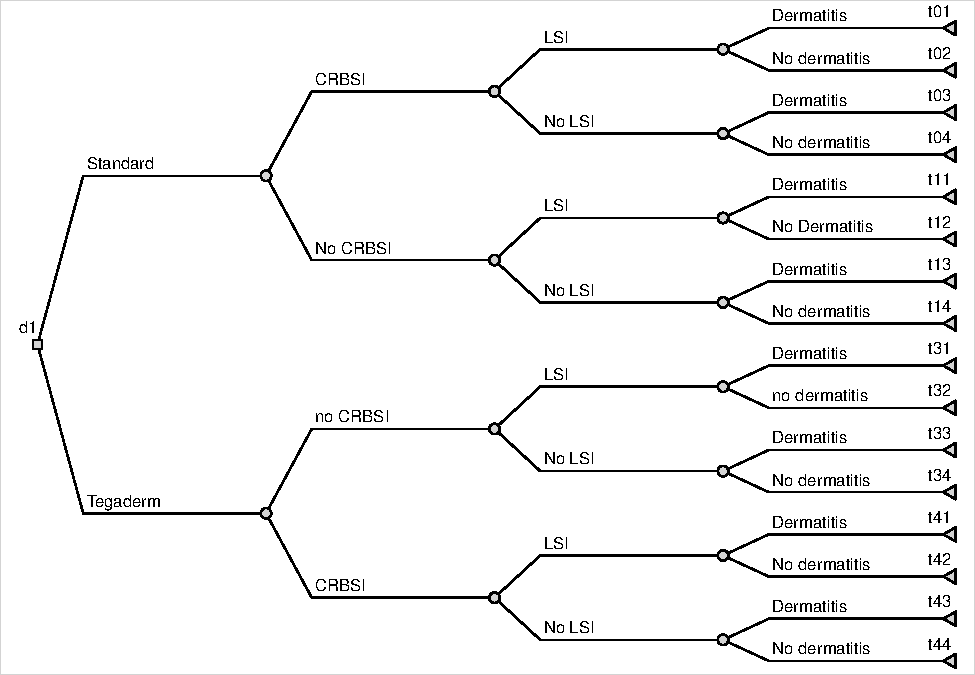
\includegraphics{DT03-ShaleGas_files/figure-latex/draw-1} \end{center}

\hypertarget{evaluating-the-strategies}{%
\section{Evaluating the strategies}\label{evaluating-the-strategies}}

There are a total of 12 possible strategies (3 choices from node
\texttt{d1} \(\times\) 2 choices at node \texttt{d2} \(\times\) 2
choices at node \texttt{d3}). But some of these are not unique. For
example if the choice at node \texttt{d1} is ``sell,'' the choices at
nodes \texttt{d2} and \texttt{d3} (4 possible combinations) are
unimportant; all four such strategies are identical. In identifying
strategies, \texttt{rdecision} discards non-unique strategies, and uses
the labels of an arbitrarily chosen strategy within each identical group
as the identifier for the strategy; i.e.~``sell/sell/sell'' also
represents the identical ``sell/sell/dig,'' ``sell/dig/sell'' and
``sell/dig/dig.''

Similarly, four strategies with choice ``dig'' at node \texttt{d1} are
identical. Removing the six repeated strategies leaves a total of six
possible strategies to evaluate.

Unique strategies are identified by \texttt{rdecision} automatically.
Method \texttt{evaluate} calculates the expected cost, benefit and
utility of each traversable path for each strategy, and aggregates by
strategy. The results for the gas problem are computed as follows.
Payoff is defined as benefit minus cost.

\begin{Shaded}
\begin{Highlighting}[]
\CommentTok{\# find optimal strategies}
\NormalTok{RES }\OtherTok{\textless{}{-}}\NormalTok{ DT}\SpecialCharTok{$}\FunctionTok{evaluate}\NormalTok{()}
\NormalTok{RES}\SpecialCharTok{$}\NormalTok{Payoff }\OtherTok{\textless{}{-}}\NormalTok{ RES}\SpecialCharTok{$}\NormalTok{Benefit}\SpecialCharTok{{-}}\NormalTok{RES}\SpecialCharTok{$}\NormalTok{Cost}
\end{Highlighting}
\end{Shaded}

This gives the following payoff for each unique strategy:

\begin{longtable}[]{@{}lllrrr@{}}
\toprule
d1 & d2 & d3 & Cost & Benefit & Payoff\tabularnewline
\midrule
\endhead
sell & sell & sell & 0 & 800 & 800\tabularnewline
dig & sell & sell & 300 & 1750 & 1450\tabularnewline
test & sell & sell & 50 & 888 & 838\tabularnewline
test & dig & sell & 134 & 895 & 761\tabularnewline
test & sell & dig & 266 & 1743 & 1477\tabularnewline
test & dig & dig & 350 & 1750 & 1400\tabularnewline
\bottomrule
\end{longtable}

The optimal strategy is test/sell/dig, \emph{i.e.} test, sell if
negative and dig otherwise. The expected payoff from this strategy is
1477.

\hypertarget{references}{%
\section*{References}\label{references}}
\addcontentsline{toc}{section}{References}

\hypertarget{refs}{}
\begin{CSLReferences}{1}{0}
\leavevmode\hypertarget{ref-kaminski:2018a}{}%
Kamiński, Bogumil, Michal Jakubczyk, and Przemyslaw Szufel. 2018. {``A
Framework for Sensitivity Analysis of Decision Trees.''} \emph{Central
European Journal of Operational Research} 26: 135--59.
\url{https://doi.org/10.007/s10100-017-0479-6}.

\end{CSLReferences}

\end{document}
